\chapter{\MATLAB{} scripts}
\thispagestyle{fancy}
\label{ch:scripts}


As you probably noticed during the previous exercises, entering \MATLAB{} commands at the prompt is a difficult way to create a structured, coherent program, especially because the order in which commands are executed is important. The solution to this problem is the \MATLAB{} script\index{script} file. The script file is a user-created text file that contains a sequence of \MATLAB{} commands that are created with the \MATLAB{} editor.
\begin{action}
Type: 
\end{action}
\prompt{edit}

\noindent The \MATLAB{} text editor window will open. In this window, you can write series of command lines, edit them and save them for running in \MATLAB{} whenever you choose to. These files are called `scripts' and are saved as *.m files\index{m-file}\index{*.m file extension}\footnote{By default, Windows XP does not show a file's extension in Windows Explorer. However, you can change the default behavior by clicking \guitext{Start} \ding{217} \guitext{Settings} \ding{217} \guitext{Control Panel}. Next, double-click \guitext{Folder options} and choose tab \guitext{View}. In the list of items, uncheck \guitext{Hide extensions for known file types}. Open Windows Explorer to confirm that it now shows the file extension.}. Whenever you type the filename of your script in the command window, the command lines in that file are executed one after the other. It is important to add comment lines\index{comment lines}\index{comment} (as opposed to `command lines') that explain the purpose of specific parts of your program. 

\hintbox{If the first character on a line is {\tt \%}, that whole line is regarded as a comment line. Comment lines are easily recognized in the \MATLAB{} m-file editor because its font color is by default set to green. Comments are ignored by \MATLAB{} during calculations.}


\noindent An example of a MATLAB script is given in \lstlistingname{}~\ref{list:florac} on page \pageref{list:florac}. Studying existing scripts is an excellent way to learn about MATLAB programming.
\lstinputlisting[float=p,caption={Calculation of evapotranspiration at Florac, France},label=list:florac]{./../m/florac.m}


\hintbox{When writing scripts, it is often helpful to structure your program according to the general structure described in \lstlistingname{}~\ref{list:general-structure}. Standardizing m-files in this way makes them easier to design, program, and interpret at a later time.}


\lstinputlisting[float=ht,caption={General structure of script m-files},label=list:general-structure]{./../m/general_structure.m}
\label{ind:initialization-part}


\noindent
\begin{minipage}[]{\textwidth}{
\centering
\vspace{2em}
\hrule
\begin{minipage}[]{0.7\textwidth}{
\vspace{2em}{\centering \begin{spacing}{1.5}{\large \textbf{From this moment on, you will develop your programs in the \MATLAB{} editor.} \end{spacing}}}\vspace{1em}
}
\end{minipage}
\hrule
\vspace{2em}
}
\end{minipage}


\begin{action}
Set the work directory to `\textbackslash{}ch05\_scripts'. Start a new script in which the assignments of the exercise below are executed, save it as `\starred{name}\_gargellen.m' in the work-directory (\starred{name} being your own last name).
\end{action}



\begin{action}
Clear the \MATLAB{} workspace by adding the appropriate command to your m-file. After saving your file, you can execute its contents by typing the script's file name at the prompt. Note that you must omit the script's extension (.m) when typing its name in the command window. Alternatively, you might want to click the `run\ldots' button in the editor (see Figure \ref{fig:run-button}).
\end{action}


\begin{figure}[!ht]
  \centering
    \fbox{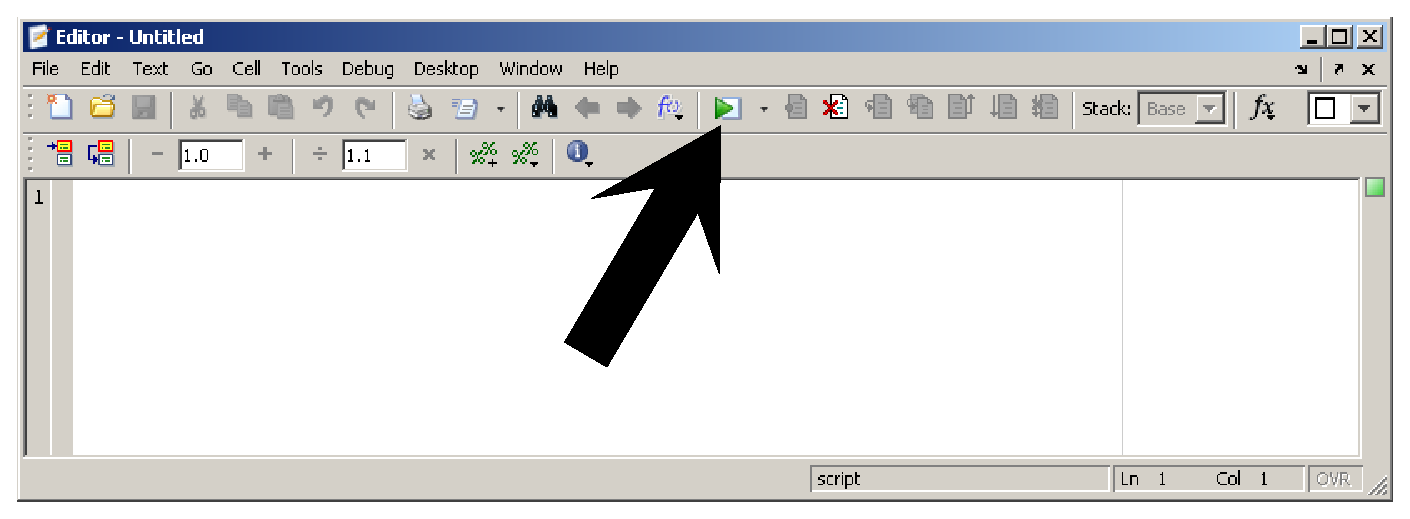
\includegraphics[width=1.0\textwidth]{./../eps/run-button.eps}}
  \caption{Location of the `run' button.}
  \label{fig:run-button}
\end{figure}


\noindent The file `demIceAge.txt' contains data on the elevation (in units of meters) of gridcells 10,000 years BP in the Gargellen valley in Austria\footnote{47.003658$^{\circ}$N,9.955546$^{\circ}$E}. 10,000 years ago, during the Ice Ages, the Gargellen Valley was under a glacier. After an increase in temperature, the ice melted and erosion created a major gully. The data file `dem2001.txt' contains the elevation (in units of meters) of the Gargellen Valley as of 2001.
\begin{action}
Load the files `demIceAge.txt' and `dem2001.txt' into the workspace. 
\end{action}




\begin{action}
Use the {\tt imagesc} command to display the contents of the variables {\tt demIceAge} and {\tt dem2001} in subplot(2,2,1) and subplot(2,2,2). Use a {\tt colorbar}\index{colorbar@\texttt{colorbar}} statement to indicate the elevation. 
\end{action}

\begin{action}
Give the subplots representative titles. 
\end{action}



\begin{action}
Calculate the difference in height between {\tt demIceAge} and {\tt dem2001} to obtain a map indicating the amount of erosion (in units of meters) over the last 10,000 years. Display this difference in subplot 3, and give it a title. 
\end{action}

\begin{action}
Given that the grid cell dimensions of both DEMs is 25 x 25 meters, calculate the total volume of rock that has been eroded in the past 10,000 years.
\end{action}

\begin{action}
Save and execute your \MATLAB{} script program.
\end{action}

\begin{action}
Before proceeding to the next project, make a review of concepts covered in Chapter \ref{ch:scripts}.
\end{action}



\hintbox{Good programming practices:
\begin{enumerate}
\item Don't forget to clear your Workspace variables when you begin to program your script files;
\item Try to limit the use of numbers in the Dynamic Part of your script (see \lstlistingname{}~\ref{list:general-structure} on page \pageref{list:general-structure}). Instead, use variables with a value that was assigned in the Initialization section;
\item Build your script by starting with the Initialization and the Output (see \lstlistingname{}~\ref{list:general-structure} on page \pageref{list:general-structure}). Then add the calculations in between;
\item Test parts of your script regularly. This is easily done by copy-pasting those parts of the script code to be tested into the \guitext{Command Window}, and then executing these parts separately. Alternatively, you can run parts of your m-file by selecting them in the editor and subsequently pressing F9 (or equivalently: right-click and choose \guitext{Evaluate Selection}).
\end{enumerate}

}%end hintbox


\project{Lead pollution in the Geul river valley}
The Geul river is located in the Province of Limburg, The Netherlands. Because of past mining activities in the area around the Geul, the river water used to contain high quantities of heavy metals including cadmium (Cd), mercury (Hg), and lead (Pb). For decades, these heavy metals have been deposited in the Geul Valley. As a result, the soil in the vicinity of the Geul river has been polluted.

The Province of Limburg wants to develop the area, but can only do so after a safety assessment has been made. Specifically, they are interested in the severity of Pb pollution in part of the valley. Cd and Hg concentrations have already been measured. These two metals do not reach dangerous concentrations and will therefore not threaten the construction plans. However, the Pb concentrations may exceed the maximum allowed concentration in parts of the valley. To investigate this, the construction companies and politicians have commissioned an assessment of the severity of the Pb pollution in the Geul valley.

More than 100 soil samples have already been taken, and a map has been constructed. Now it's up to you to manipulate and analyze this data. First, let's take a look at the Geul lead pollution data. The data are available as `geulmap.txt'. 

\begin{action}
Make sure you follow the m-file standardization guidelines for this project (see \lstlistingname~\ref{list:general-structure} on page \pageref{list:general-structure} and the Tip above). Set your work directory to `\textbackslash{}ch05\_scripts\textbackslash{}proj04\_geul' for this exercise.
\end{action}

\begin{action}
Start the m-file editor and save the empty script program as `\starred{name}\_geul.m' (with your name for \starred{name}) in your new work directory.
\end{action}

\begin{action}
Load the geulmap data into your \MATLAB{} workspace. Use {\tt imagesc} and {\tt colorbar} commands to have a quick look at the Geul river data. Let your script visualize the {\tt geulmap} data in the upper left subplot (see Figure~\ref{fig:geul}).
\end{action}




%It's important to note that the dark blue areas represent areas of zero lead concentrations. In fact no measurements were taken here. However, because these areas are much higher than the Geul river, it's assumed that there are no hazardous lead concentrations in these areas. Thus, these zero-value grid cells are not part of the Geul valley under investigation, but are included in development areas.


\begin{action}
Initially, the plan is to clean all grid cells which have concentrations in excess of 350 mg/kg. Make a 2-D logical array {\tt concMoreThan350} which is {\tt true} for indices in {\tt geulmap} that are greater than 350. Let your script visualize it in the lower right subplot. 
\end{action}

\begin{action}
Let your program calculate the total cost of having to clean all cells with concentrations in excess of 350 mg/kg, when given that the area of one grid cell is 900 m$^2$, and the cost equation for one grid cell is:
\end{action}
\begin{equation} 
TotalCost = 1000 + 1.7031 \times CellArea
\end{equation}
where $TotalCost$ is the cost in euro, and $CellArea$ is the grid cell area in m$^2$. (The correct answer is \euro~23719578).

\begin{action} 
Let your program round off the total cost to the nearest euro (see {\tt doc round}).
\end{action} 

\begin{action}
Just as you used concatenation\index{concatenation} to merge numeric arrays (see Chapter~\ref{ch:concatenation} on page~\pageref{ch:concatenation}), you can also let \MATLAB{} merge character arrays. At the prompt, create the character array {\tt string1}:
\end{action}
\prompt{string1 = \squote{My age is: }}
\noindent Now, create the \textul{character} array:
\prompt{myAge = \squote{29}}
\noindent (Note the quotes). At this point, you can merge the two strings by:
\prompt{stringBoth = [string1,myAge]}
\noindent However, you'll often find that you want to merge a character array with a numeric array, rather than two character arrays. If {\tt myAge = 29} rather than {\tt myAge = \squote{29}},
\prompt{stringBoth = [string1,myAge]}
\noindent will not yield the proper result. We can solve this by using the {\tt num2str}\index{num2str@\texttt{num2str}} function, which is used to convert numeric values to their character array respresentation.

\noindent For example, try out the following:
\prompt{clear}
\prompt{string1 = \squote{My age is: }}
\prompt{myAge = 29}
\prompt{stringBoth = [string1,num2str(myAge)]}

\begin{action}
Now let your program create a title similar to the one in the lower right subplot of Figure~\ref{fig:geul} on page~\pageref{fig:geul}.
\end{action}

\vspace{1em}
\noindent It turns out that the 350 mg/kg level was a bit too ambitious: the Province does not want to spend more than 14 million euro on cleaning the soil. It has therefore been decided that the best solution is to clean those parts where humans will be exposed to the soil (recreational areas, playgrounds and so on). After these so-called priority areas have been cleaned, the rest of the money will be used to clean as much of the valley as possible; for this part of the operation, the goal is to clean all grid cells which have a Pb concentration above a certain level.
\vspace{1em}

\begin{action}
Load the priority areas from the file `needs-cleaning.mat'. Visualize the array in the upper right subplot. Give it an appropriate title.
\end{action}

\noindent At this point, your program can visualize a logical array of concentrations above a certain level, and it can also display the logical map containing the priority areas. However, before we proceed with the project, let's digress for a moment to take a look at logical expressions (as you will see later, these are useful for the completion of the Geul project). After that, we'll come back to the Geul river project to finish up.


\section{Logical expressions}
Earlier on, we encountered relational expressions such as {\tt A$>$8}, or {\tt B$\sim=$C}. However, sometimes you want to test for more complicated relations. This is when logical expressions come in handy. Basically, there are 4 logical expressions (see also Figure~\ref{fig:logical-expressions} for a graphical explanation):
\begin{table}[ht]
\vspace{1em}
\caption{Logical expressions.}
\label{tab:logical-expressions}
\vspace{-0.5em}
\centering
\begin{tabular}{|l|c|p{8cm}|}
\hline
\textbf{Expression}&\textbf{Sign}&\textbf{Description}\\
\hline
AND&\verb#A&B#\index{\&}&The AND expression combines entries from logical arrays {\tt A} and {\tt B}, returning {\tt true} if and only if an element in {\tt A} is {\tt true} and the same element in {\tt B} is also {\tt true}.\\
\hline
OR&\verb#A|B#\index{\mid}&The OR expression combines entries from logical arrays {\tt A} and {\tt B}, returning {\tt true} if an element in {\tt A} is {\tt true} or the same element in {\tt B} is {\tt true} or when they are both {\tt true}.\\
\hline
Exclusive OR&\verb#xor(A,B)#\index{xor@\texttt{xor}}&The Exclusive OR expression combines entries from logical arrays {\tt A} and {\tt B}, returning {\tt true} if an element in {\tt A} is {\tt true} or the same element in {\tt B} is {\tt true}. It returns {\tt false} if the element is {\tt true} in both array {\tt A} and {\tt B}.\\
\hline
NOT&$\sim${\tt A}\index{$\sim$}&The NOT expression negates the values in {\tt A}, that is, what is {\tt true} will become {\tt false}, and vice versa. Is equivalent to {\tt A==0} when {\tt A} is logical.\\
\hline
\end{tabular}
\end{table}



\begin{figure}[!htb]
  \centering
    \fbox{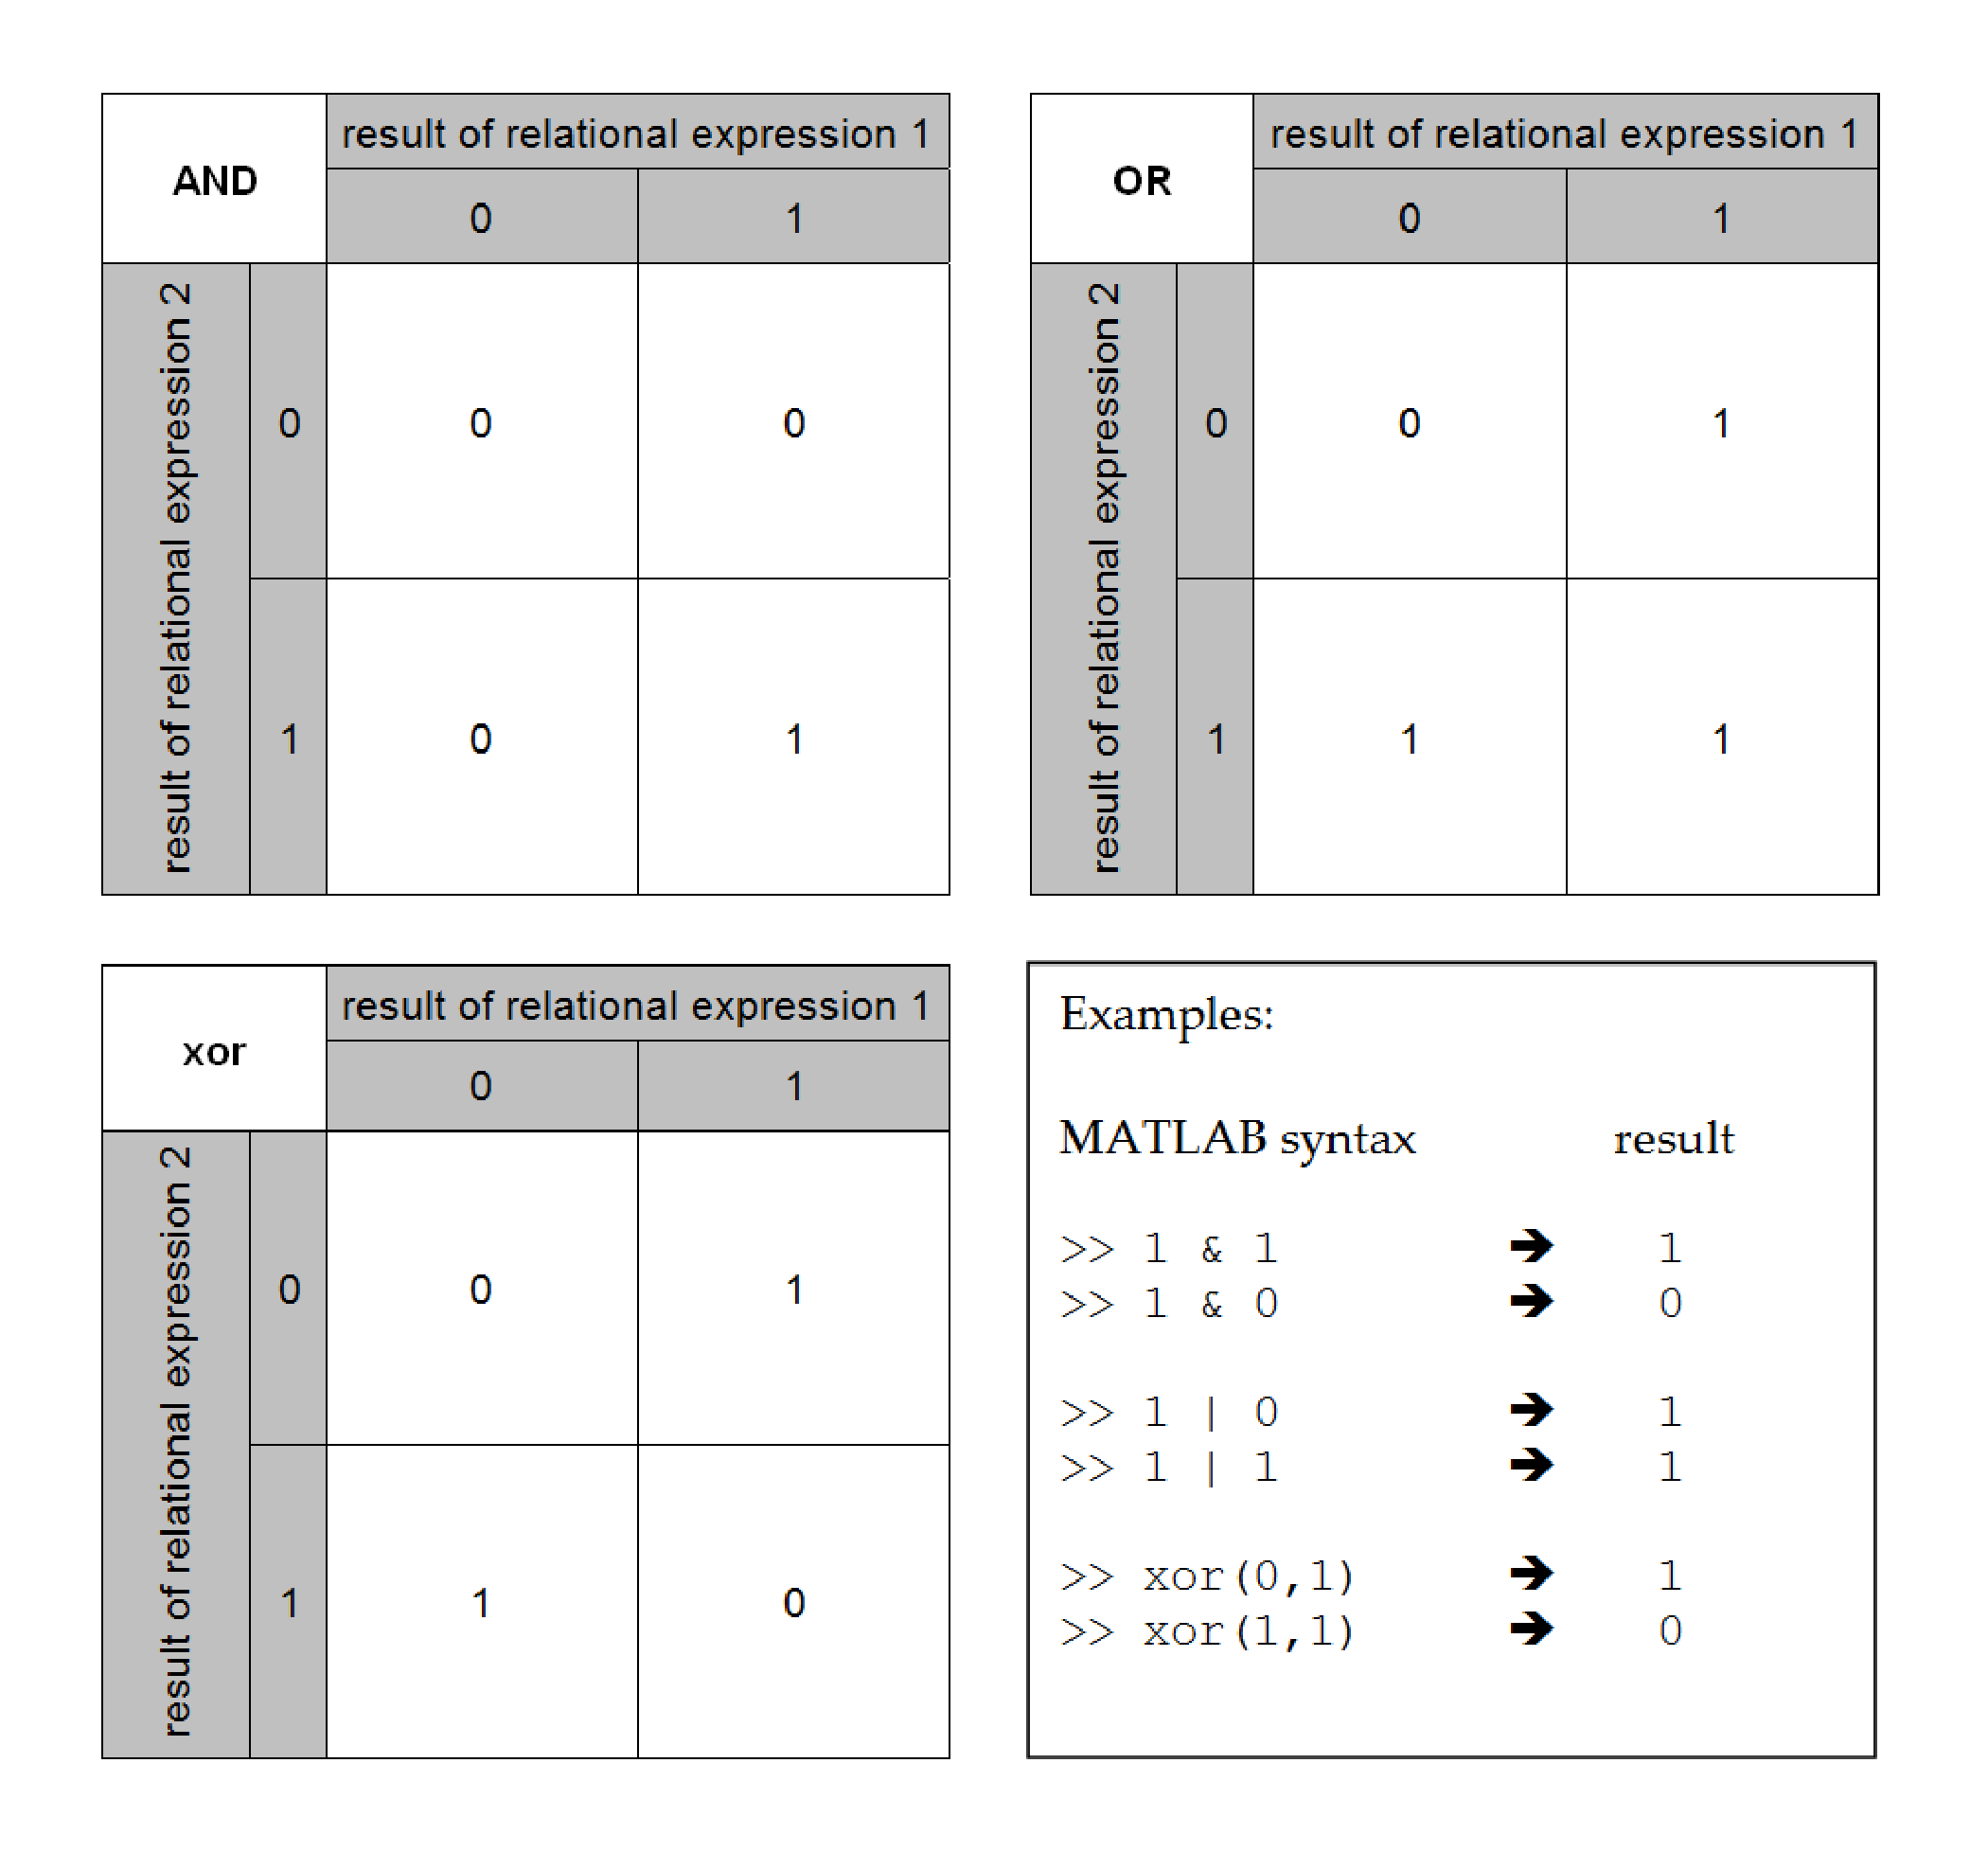
\includegraphics[width=1.0\textwidth]{./../eps/logical.eps}}
  \caption{Logical expressions.}
  \label{fig:logical-expressions}
\end{figure}


\begin{action}
Clear your workspace
\end{action}

\begin{action}
Type
\prompt{A = [2,8,0,4,3,10];}
\end{action}

\begin{action}
Type
\prompt{M = (A > 3) \& (A < 10)}
\end{action}
\begin{action}
Why would the OR-operator be useless in this example? What would be the result? 
\end{action}

\hintbox{Relational and logical operations can only be performed if the arrays are of the same size.}


\begin{action}
With this new knowledge of combining logical arrays, go back to your Geul script. What is the logical expression which allows you to create an array that has {\tt true} on all positions that need to be cleaned? (Remember that cleaning is necessary in case of high Pb concentration, or because it's a priority area).
\end{action}
\begin{action}
If you didn't already do this, change your script in such a way that you can recalculate the total cost of cleaning by changing the value of 1 variable in your program.
\end{action}
\begin{action}
Adjust the value of this variable until it meets the budget as set by the Province of Limburg, while maximizing the cleaning objective.
\end{action}


\section{Saving your variables to file}

\begin{action}
You can let \MATLAB{} save workspace variables to harddisk. For example, typing
\prompt{save(\squote{testfile.mat})}\index{save@\texttt{save}}
will save all variables that are present in the workspace to a so-called `$\ast{}$.mat-file' (extension\index{file extension} is .mat, file type is binary) which you can load at a later time.
\end{action}

\begin{action}
Execute the current exercise in the command window: Create some arbitrary variables and save them to a $\ast{}$.mat file. Now issue a {\tt clear} command. Check that your workspace is now empty. Next, load the $\ast{}$.mat file into the workspace. Check the workspace again.
\end{action}

\noindent Because it is usually unnecessary to save all the variables in your workspace to harddisk, you can also save specific variables only. If you want your files to be saved as text files instead of binary files, you must use the {\tt save} option {\tt \squote{�ascii}} to indicate the desired file format. If you choose to use the ASCII text format, your filename should have the `*.txt' extension. The {\tt save}  command can be incorporated in your script files just like any other command.

\vspace{1em}

\noindent Although the {\tt save} command can be used in a number of ways (see {\tt doc save}), its most common forms are:
\begin{lstlisting}[numbers=none]
save('safemap.txt','SafeMap','-ascii')
\end{lstlisting}
and
\begin{lstlisting}[numbers=none]
save('valley-variables.mat','SafeMap','ValleyIO','gridCellArea')
\end{lstlisting}

\noindent The first example saves the variable {\tt SafeMap} to a file `safemap.txt' containing plain text (ASCII\index{ASCII}\footnote{\url{http://en.wikipedia.org/wiki/ASCII}} essentially means `unformatted text'. You may be familiar with files that you can read with Notepad --these are ASCII files). Remember that variable names are not allowed to start with anything but a letter character (see TIP on page \pageref{tip:naming-conventions}); this way, \MATLAB{} knows that {\tt \squote{-ascii}} must be an option rather than a variable. The second example saves the 3 variables to the binary file `valley-variables.mat'. Check the \MATLAB{} help documentation for further information on the {\tt save} command.

\begin{action}
Let your program save the most important variables to a file on harddisk.
\end{action}



\begin{figure}[!htb]
  \centering
    %\fbox{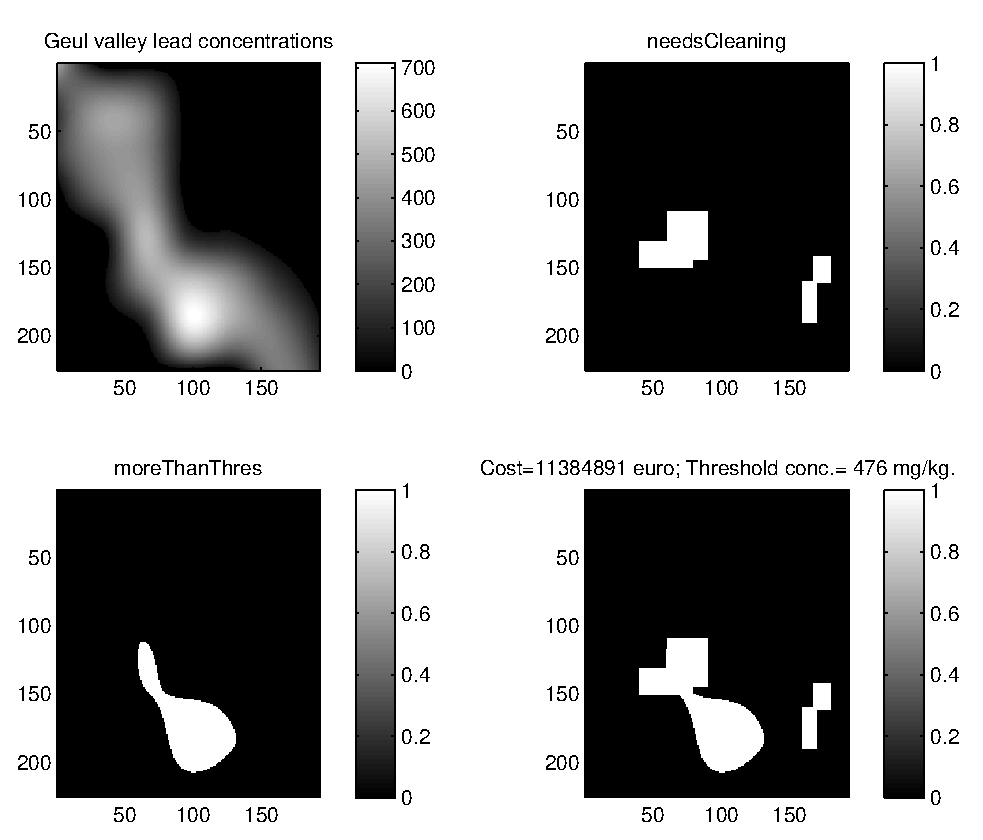
\includegraphics[width=1.0\textwidth]{./../eps/geul.eps}}
    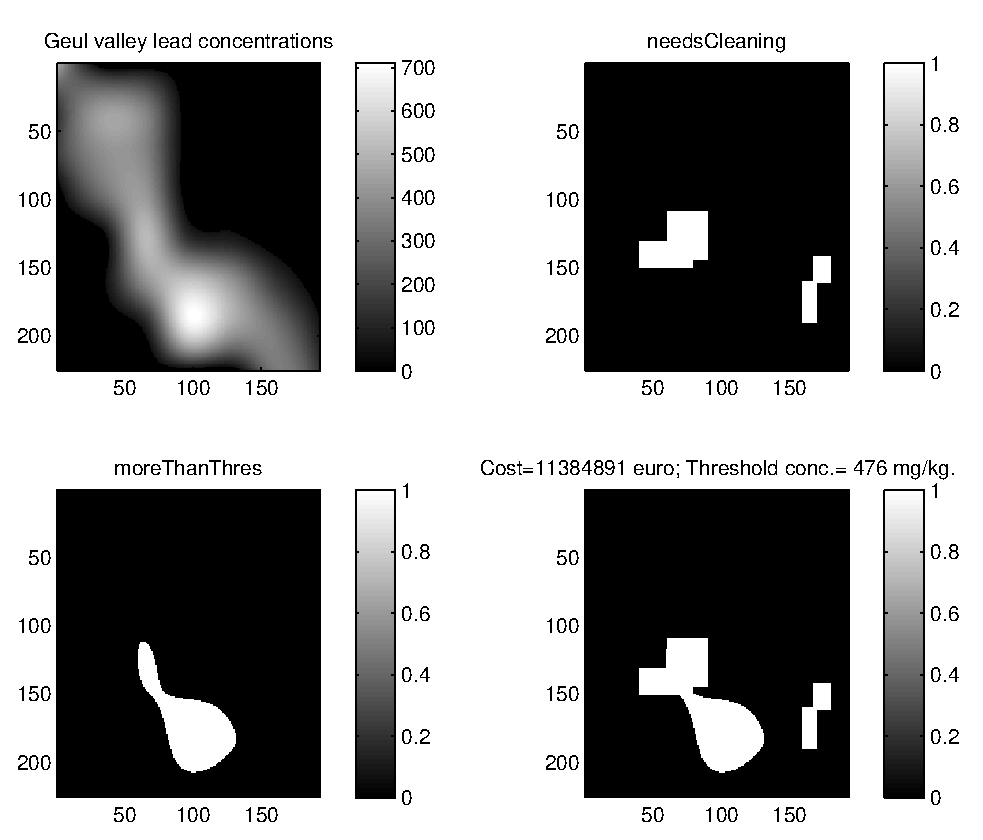
\includegraphics[width=1.0\textwidth]{./../eps/geul.eps}
  \caption{End result of the Geul pollution project. Note that the colors are different to facilitate easier interpretation when printed.}
  \label{fig:geul}
\end{figure}
\vspace{-2em}
\projectfooter
